\Problem
{تمایز \lr{CSMA}، \lr{CSMA/CD} و \lr{CSMA/CA}}
{
\lr{Carrier Sense Multiple Access}
یا
\lr{CSMA}
یک روش برای حل مشکل دسترسی چندگانه است که مبتنی بر مکانیزم
\lr{CSM}
کار می‌کند.
این روش برای کاهش احتمال تصادم میان کاربران توسعه داده شد.
در این روش هر کاربر ملزم به چک کردن رسانه قبل از ارسال سیگنال است.
در واقع هر کاربر باید وضعیت حامل را جویا شود.
دو روش دیگر مبتنی بر همین روش ایجاد شده اند که یکی بر روی جلوگیری از تصادم و دیگری روی تشخیض تصادم تمرکز دارد.

\lr{CSMA with Collision Detection}
یا
\lr{CSMA/CD}
روشی است که کاربر پس از ارسال داده همچنان رسانه را مورد بررسی قرار می‌دهد تا مطمئن شود که انتقال موفقیت آمیز بوده است.
اگر انتقال موفقیت آمیز باشد کار کاربر تمام است. در غیر این صورت کابربر داده را دوباره ارسال می‌کند.

\begin{figure}[H]
    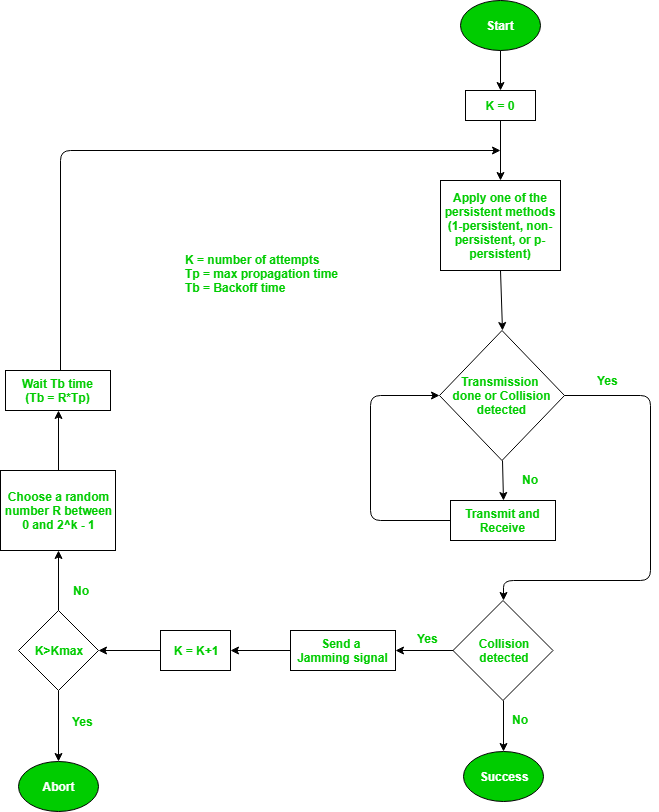
\includegraphics[width=9cm]{Images/CSMA_CD.png}
    \centering
    \caption{\lr{CSMA/CD Flow}}
\end{figure}


\lr{CSMA with Collision Avoidance}
یا
\lr{CSMA/CA}
روشی مبتنی بر این ایده است که ایستگاه مخابراتی باید بتواند همزمان با ارسال اطلاعات جهت تشخیص تصادم، اطلاعاتی را نیز از ایستگاه‌های مختلف دریافت کند.
این روش به خصوص در شبکه‌های بیسیم کاربرد دارد زیرا انرژی سیگنال دریافتی تقریبا دو برابر می‌شود و به راحتی می‌توان تصادم را تشخیص داد.

\begin{figure}[H]
    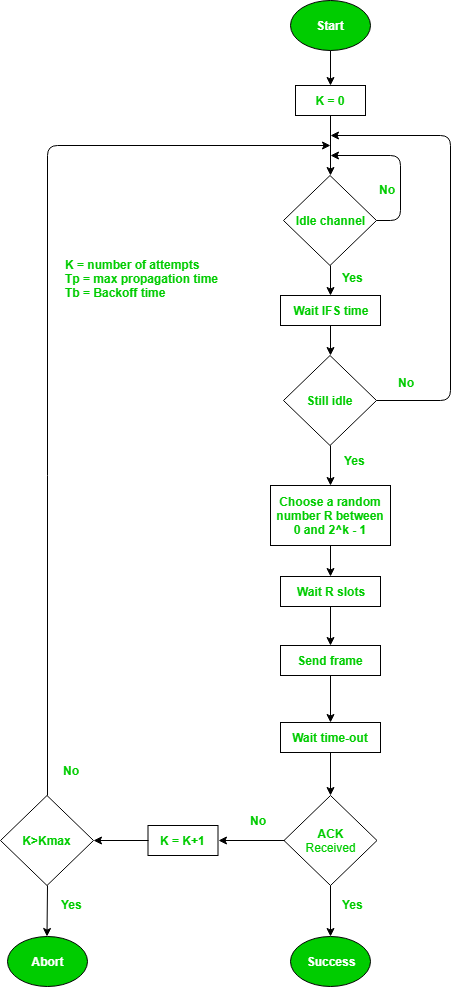
\includegraphics[width=8cm]{Images/CSMA_CA.png}
    \centering
    \caption{\lr{CSMA/CA Flow}}
\end{figure}

\begin{itemize}
    \item
    اولی بعد از تصادم موثر است، دومی قبل از تصادم موثر است.
    
    \item
    اولی در شبکه‌های باسیم بکار می‌رود، دومی عموما در شبکه‌های بی‌سیم بکار می‌رود.
    
    \item
    نتیجه اولی کاهش زمان ریکاوری است، در صورتی که دومی احتمال تصادم را کاهش می‌دهد.
    
    \item
    اولی در صورت رخداد تصادم داده را باز ارسال می‌کند، در صورتی که در دومی اینطور نیست.
    
    \item
    اولی در استاندارد 
    \lr{802.3}
    بکار رفته، در صورتی که دومی در استاندارد
    \lr{802.11}
    استفاده شده است.
    
    \item
    روش
    \lr{CSMA/CD}
    بسیار موثر‌تر از روش
    \lr{CSMA}
    ساده است.
    
    \item
    روش
    \lr{CSMA/CA}
    بسیار شبیه به روش
    \lr{CSMA}
    ساده است.
\end{itemize}
}
